

\ccAnchor{http://qt.nokia.com/}{Qt} is a {\sc Gui} toolkit for
cross-platform application development.

% +-----------------------------------------------------+
\section{Introduction}

This chapter describes classes that help to visualize two dimensional \cgal\ objects
with the \ccAnchor{http://doc.qt.nokia.com/latest/graphicsview.html}{Qt Graphics View Framework}.

This framework uses the model view paradigm. \ccAnchor{http://doc.qt.nokia.com/latest/qgraphicsitem.html}{\ccc{QGraphicsItem}}s are stored in a 
\ccAnchor{http://doc.qt.nokia.com/latest/qgraphicsscene.html}{\ccc{QGraphicsScene}} 
and are displayed in a \ccAnchor{http://doc.qt.nokia.com/latest/qgraphicsview.html}{\ccc{QGraphicsView}}. The items 
have a paint method which is called when an item is in the visible area of a view.
The framework is also responsible for dispatching events from the view
via the scene to the items. The framework is extensible in the sense
that users can add classes derived from \ccc{QGraphicsItem}.

Besides visualizing \ccc{QGraphicsItem}s users want to enter geometric objects.
We provide the input generators for all 2D \cgal\ kernel objects.

The package includes also a class for providing zooming, panning, and scrolling
to the graphics view.


The following sections describe the interaction between all these classes,
We finally describe the internals of a \ccc{QGraphicsItem}.

\subsection{Naming Conventions}

As Qt and \cgal\ have different naming conventions, and as this package
brings them together we adopted the following, hybrid naming conventions.

\begin{itemize}
\item All header files are in the directory \ccc{CGAL/Qt/}. 
\item Class names are concatenated capitalized words, and function names are
      concatenated capitalized word with the first word in lowercase. The rationale is that
      these classes are related to Qt, and that they sometimes are derived
      classes that have to override member functions adhering to this naming scheme.
\item All classes are in the nested namespace \ccc{CGAL::Qt}.
\end{itemize}
 


\section{Overall Design}

In Figure~\ref{graphicsview:uml} you see four classes depicted in grey,
that come from the Qt Graphics View Framework. The \ccAnchor{http://doc.qt.nokia.com/latest/qgraphicsscene.html}{\ccc{QGraphicsScene}}
contains \ccAnchor{http://doc.qt.nokia.com/latest/qgraphicsitem.html}{\ccc{QGraphicsItem}}s, which get displayed in any number
of \ccAnchor{http://doc.qt.nokia.com/latest/qgraphicsview.html}{\ccc{QGraphicsView}}s. The views are widgets, that is they take screen space
in an application.

The fourth class is the \ccAnchor{http://doc.qt.nokia.com/latest/qobject.html}{\ccc{QObject}}. It plays an important role in Qt for
event handling and memory management. First, it allows to add \ccAnchor{http://doc.qt.nokia.com/latest/signalsandslots.html}{signals and
slots}, and to connect them.  Second, it allows to install \ccAnchor{http://doc.qt.nokia.com/latest/eventsandfilters.html}{event filters}.


\begin{figure}[t]
\begin{ccTexOnly}
  \begin{center}
  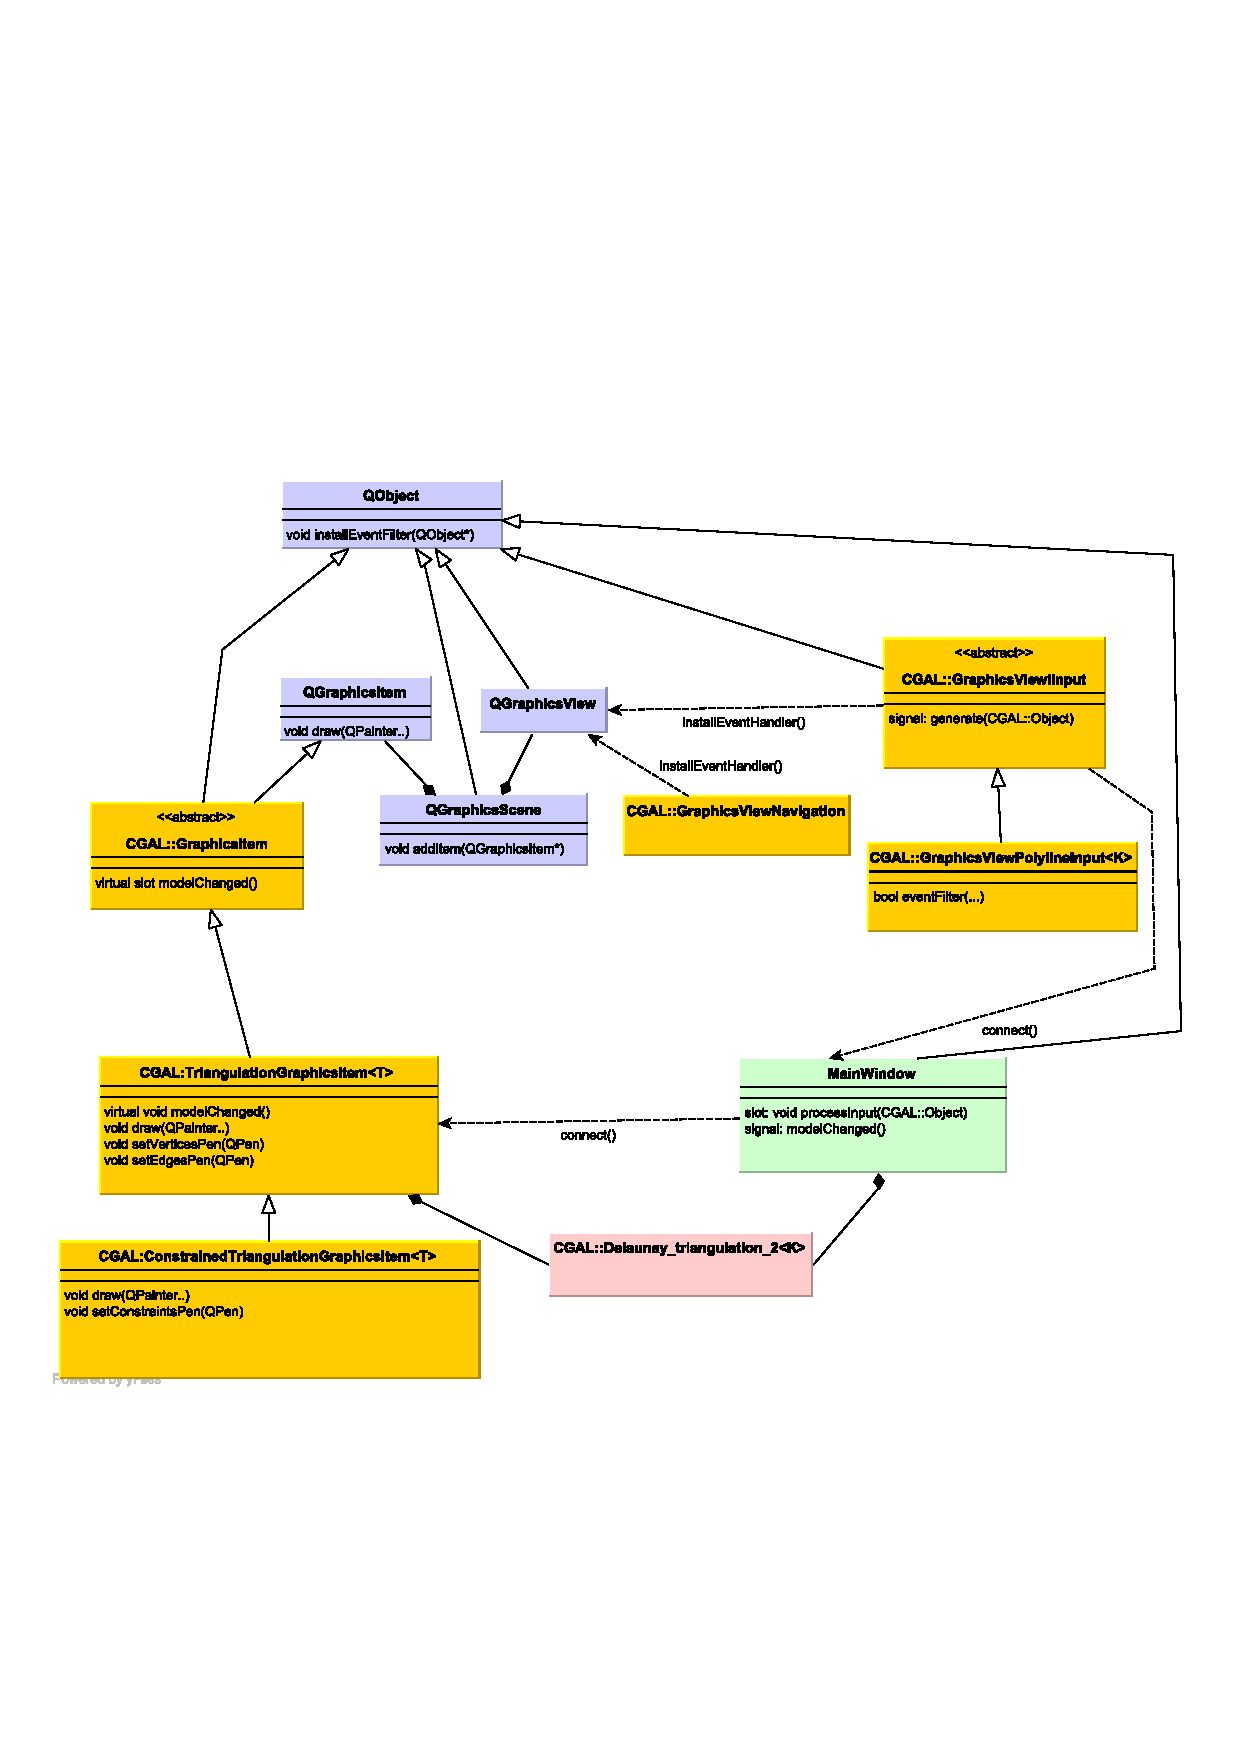
\includegraphics[width=\linewidth]{GraphicsView/uml-design}
  \end{center}
\end{ccTexOnly}
\begin{ccHtmlOnly}
  <p><center>
  <img src="./uml-design.png" border=0 alt="UML Class Diagram">
  </center>
\end{ccHtmlOnly}
\caption{UML Class Diagram with the Qt classes (blue), \cgal\ classes for using the framework (yellow),
\cgal\ data structures (red), and application classes (green). \label{graphicsview:uml}}
\end{figure}

\subsection{Visualizing CGAL Datastructures}

In order to visualize for example a \ccc{CGAL::Delaunay_triangulation_2<K>}, we
provide the graphics item class \ccc{CGAL::Qt::TriangulationGraphicsItem<T>}.
It provides a \ccc{paint} method that draws the edges and vertices of a triangulation
using the drawing primitives of the \ccc{QPainter}.   The color of vertices and edges, 
can be chosen by setting a user defined  \ccc{QPen}.


As this graphics item only stores a pointer to a triangulation, it
must be notified about changes like the insertion of points coming from
a file, a process or as input generated with the mouse.  We
use the signal/slot mechanism of Qt for that purpose, that is when the
triangulation changes the application emits a signal that can get connected to the
\ccc{modelChanged()} slot of the graphics item.



\subsection{Navigation}

We provide a class \ccc{CGAL::Qt::GraphicsViewNavigation} that can be
installed as an event filter of a graphics view and its viewport. As for
all Qt widgets, the \ccc{QGraphicsView} is derived from
\ccc{QObject}. Events like the  mouse buttons pressed or released, the mouse movemed, keys pressed, 
are passed to the view which first hands them over to the
event filter.  The \ccc{CGAL::Qt::GraphicsViewNavigation} event filter allows to zoom, scroll, and recenter.
Finally, the class emits a signal with the mouse coordinates. This can be used
to display the current mouse position in the status bar of an application.

\subsection{Generation of Input}

Input of \cgal\ kernel objects, polylines, etc. is generated by classes derived
from \ccc{CGAL::Qt::GraphicsViewInput}.  As the navigation class, they are event handler of the
graphics view, because they have to know where the mouse is, when the user clicks
in order to enter a point.

Once the input generator has assembled the object, which can involve several mouse clicks,
it emits a \ccc{CGAL::Object} wrapping the input.  The emitted input can be connected
by the application developer to a slot. In the 2D demos of \cgal, which use the 
Graphics View Framework we connect it to the slot \ccc{MainWindow::processInput(CGAL::Object)}.
This method unwraps from the \ccc{CGAL::Object} and inserts it in the data structure. 
It then typically emits a signal \ccc{modelChanged()} which can be 
connected to the graphics item representing the data structure.

All input generators we provide use the left mouse button for entering points.
The right click terminates a sequence of entered points. 'Delete' and 'backspace'
remove the last entered point. 'Esc' resets the input generator.  As the 'Ctrl' key
is used by the \ccc{CGAL::Qt::GraphicsViewNavigation} this modifier is not used.  

%The 'Shift' key is used for generation of axis aligned segments, rays, and lines. 

